\documentclass[xcolor=pdftex,x11names,table,hyperref]{beamer}

\usepackage{verbatim}
\usepackage{setspace}
\usepackage{graphbox}
\usepackage{url}
\usepackage{xcolor} % See documentation PDF at http://www.ctan.org/pkg/xcolor
\definecolor{darkgreen}{rgb}{0,0.3,0}
\definecolor{darkblue}{rgb}{.05,.05,.30}
\definecolor{lightgrey}{rgb}{0.65,0.65,0.65}
\usepackage{tikzsymbols}


\setbeamertemplate{section in toc}[sections numbered]
\setbeamertemplate{subsection in toc}[subsections numbered]
\setbeamertemplate{subsubsection in toc}[subsubsections numbered]
\usetheme{Singapore}
\setbeamertemplate{navigation symbols}{}
\setbeamertemplate{footline}{%
\vspace{0.0em}%
\hspace{0.5em}%
{\color[rgb]{.1,.1,.1} \insertframenumber{}~/~\inserttotalframenumber}
}

\newcommand{\code}[1]{{\color{darkgreen}\texttt{#1}}}
\newcommand{\detail}[1]{{\color{lightgrey}\small{}#1}}
\newcommand{\teeny}[1]{\scalebox{0.17}{#1}}
\newcommand{\tablecolors}{\rowcolors{2}{blue!12}{white}} % Cool table colors

\newcommand{\actfun}[1]{\includegraphics[height=0.11\textheight,align=c]{images/#1}} % For consistency

\begin{document}

\title{Neural Networks \\[1.5em]
 %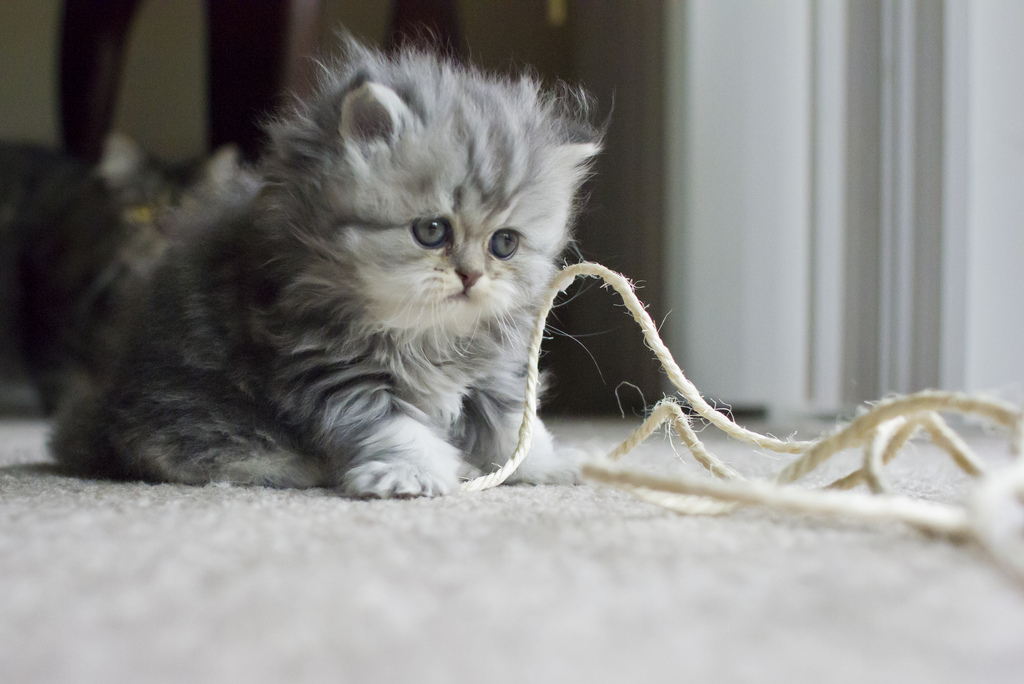
\includegraphics[width=0.5\textwidth]{images/kitten_string_flickr_albaraa.jpg} \\[-1.0em]
 \small{Part 1} \\[1.0em]
 %LT1 \\[1.0em]
 }
\author{\href{http://jon.dehdari.org}{Jon Dehdari}}
\frame{\titlepage}

%\begin{frame}{Good Morning!}
%	\begin{center}
%	%\includegraphics[width=0.8\textwidth]{images/.jpg}
%	\end{center}
%\end{frame}

% extension of maxent models
\begin{frame}{Extending Logistic Regression (=Softmax Regression)}
\begin{itemize}
	\item {\small Recall that \textbf{logistic regression} involves the dot product of an input vector and a weight matrix, then a normalized sigmoid function (softmax)}
	\pause
	\item A \textbf{feedforward neural network} just adds one or more layers between the input vector and the softmax output
	\pause
	\begin{center}
	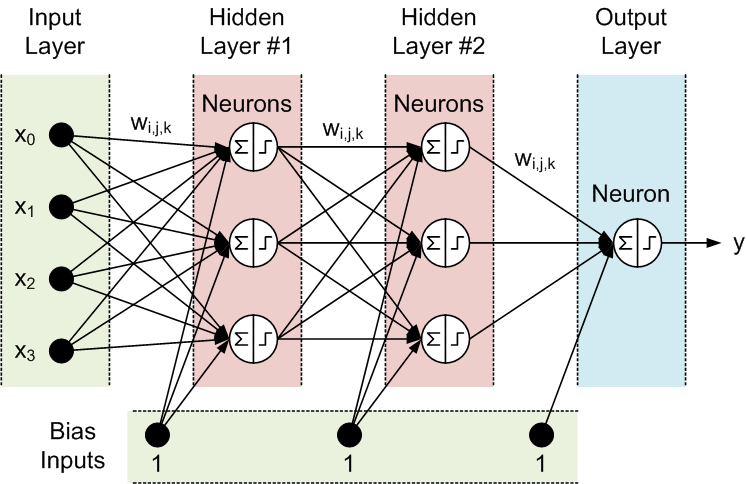
\includegraphics[height=0.58\textheight]{images/nnet_mql5.png}
	\end{center}
\end{itemize}
\teeny{Courtesy of \href{https://www.mql5.com/en/code/9002}{mql5.com}}
\end{frame}

% what can they do that maxent can't: 
% Universal approximation theorem (George Cybenko, 1989) non-linear representations.  One hidden layer: any continuous function. Two hidden layers: any discontinuous function
% https://www.mql5.com/en/code/9002
\begin{frame}{Why Use Hidden Layers?}
\begin{itemize}
	\item In contrast to log-linear models, neural networks can have \textbf{non-linear} representations of data
	\item The \textbf{\href{https://en.wikipedia.org/wiki/Universal_approximation_theorem}{universal approximation theorem}} (George Cybenko, 1989) found that a neural network with one hidden layer can approximate \textbf{any continous function}
	\item A network with two hidden layers can represent discontinuous functions
	\begin{center}
	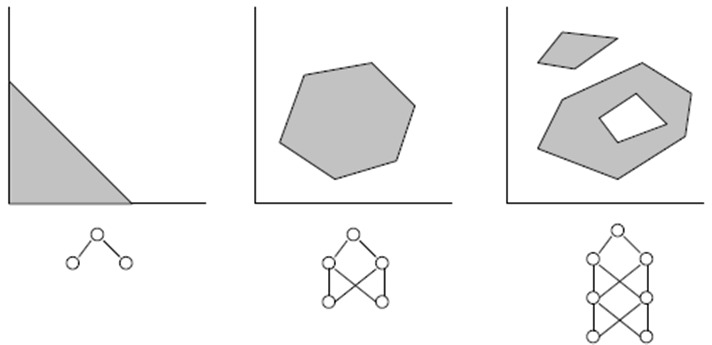
\includegraphics[height=0.42\textheight]{images/nnet_mql5_function_approximations.png}
	\end{center}
\end{itemize}
\teeny{Courtesy of \href{https://www.mql5.com/en/code/9002}{mql5.com}}
\end{frame}

% activation functions: linear, relu, heaviside step function, tanh, logistic, softmax
\begin{frame}{Activation Functions ($\sigma$)}
	In each layer, the output of the dot product goes through an \textbf{\href{https://en.wikipedia.org/wiki/Activation_function}{activation function}} ($\sigma$). Here are some examples: \\[0.3em]
\begin{footnotesize}
\begin{spacing}{0.85}
\hspace*{-3.0em}%
\begin{tabular}{lllp{0.38\textwidth}}
	\bf Name & \bf Visualization & $\bf f(x)=$ & \bf Notes \\
	\hline
	Linear  (= Identity) & \actfun{activation_linear_wp.png} & $x$ & Not useful for hidden layers \\
	Heaviside Step & \actfun{activation_heaviside_step_wp.png} & {\tiny $ \left \{\begin{array}{rcl} 0 & \mbox{if} & x < 0\\ 1 & \mbox{if} & x \ge 0\end{array} \right. $ }  \hspace*{-1.0em} & Not differentiable \\
{\scriptsize Rectified Linear (ReLU)} & \actfun{activation_relu_wp.png} & {\tiny $ \left \{\begin{array}{rcl} 0 & \mbox{if} & x < 0 \\ x & \mbox{if} & x \ge 0\end{array} \right.$ } \hspace*{-1.0em} & Surprisingly useful in practice \\
	Tanh & \actfun{activation_tanh_wp.png} & $\frac{2}{1+e^{-2x}}-1$ & A soft step function; ranges from -1 to 1 \\
	Logistic (`sigmoid') & \actfun{activation_logistic_wp.png} & $\frac{1}{1+e^{-x}}$ & Another soft step function; ranges from 0 to 1 \\
	Softmax & \actfun{activation_logistic_wp.png} & $\frac{e^{\boldsymbol W_y \cdot \mathbf{x}} }{Z} $ & Normalized sigmoidal function. Useful for last layer when training on cross entropy \\
\end{tabular}
\end{spacing}
\end{footnotesize}
\pause
{\tiny \href{http://keras.io/activations}{List of activation functions in Keras: \texttt{keras.io/activations}}}\\
\teeny{Images courtesy of \href{https://en.wikipedia.org/wiki/Activation_function}{Wikipedia}}
\end{frame}

\begin{frame}{Training Neural Networks}
\begin{itemize}
	\item At a high level, the weights in a neural net are set by means of the blame game -- whenever it guesses incorrectly, change the weights that were the most responsible for making that guess
	\pause
	\item Whenever the network guesses a training instance correctly, don't change anything
	\pause
	\item The weights are usually trained by a form of the gradient descent optimization algorithm
	\item The gradients are calculated by error \textbf{backpropagation}
	\item First, do a normal forward pass through the network, to determine the \textbf{error/loss} (how different the output was from the `correct' answer)
	\item Then, do a backwards pass (end to start), changing the weights to minimize errors
\end{itemize}
\end{frame}

\begin{frame}{Loss / Objective Functions}
\begin{itemize}
	\item \textbf{Discrete Outputs}:
	\begin{itemize}
		\item Binary Cross-Entropy (0-1 loss): 0 if correct, 1 if incorrect
		\item Categorical Cross-Entropy: good old cross-entropy. Eg.\\ 0 if $p(y)=1.0$, \\ 1 if $p(y) = 0.5$, \\ 2 if $p(y)=0.25$, \\ 3 if $p(y)=0.125$, \\ ...
	\end{itemize}
	\item \textbf{Continuous Outputs}:
	\begin{itemize}
		\item Mean Squared Error (MSE): $\frac{1}{n} \sum_{i=1}^n (\hat{y}_i - y_i)^2$
		\item Root Mean Squared Error (RMSE): $\sqrt{MSE}$
		\item Mean Absolute Error (MAE): $\frac{1}{n} \sum_{i=1}^n |\hat{y}_i - y_i|$
	\end{itemize}
\end{itemize}
\pause
\vspace*{1.0em}
\href{http://keras.io/objectives}{List of loss functions in Keras: \texttt{keras.io/objectives}}
\end{frame}

\begin{frame}{Autoencoders}
\begin{itemize}
	\item An \textbf{autoencoder} is a neural network where the size of the output layer is the same size as the input layer
	\item The hidden layers are usually smaller
	\item The goal is to generalize the training data
	\item Since no labeled data is necessary, autoencoders are an unsupervised learning technique
	\item Autoencoders trained on language data are neural language models
	\pause
	\item Autoencoders are occasionally called \href{https://en.wikipedia.org/wiki/Diabolo\#History_and_etymology}{diabolo networks} \\
	\begin{center}
	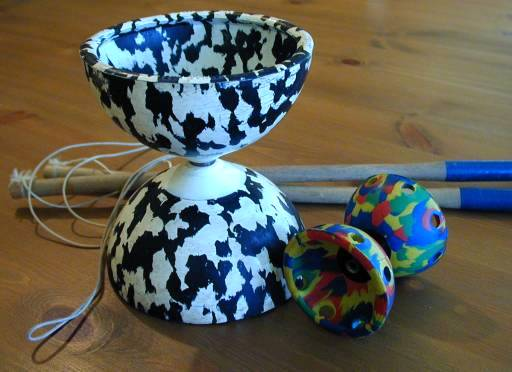
\includegraphics[height=0.35\textheight]{images/diabolo_large_and_small.jpg}
	\end{center}
\end{itemize}
\teeny{Image courtesy of \href{https://commons.wikimedia.org/wiki/File:Diabolo_large_and_small.jpg}{Wikimedia}}
\end{frame}

\begin{frame}{Tips \& Tricks (discussed in class)}
\begin{itemize}
	\item Network depth
	\item Layer size
	\item Dropout
	\item Early stopping
	\item Optimizers
	\item Learning rate
\end{itemize}
\end{frame}

% software: theano-based, tensorflow-based, torch-based, others (Caffe, DL4J, CNN, ...)
\begin{frame}{Software}
\begin{itemize}
	\item Most popular neural net software are based on the following: \\[1.0em]
\hspace*{-2.0em}%
\begin{tabular}{llll}
	\bf Name & \bf Lang Support & \bf GPU Support & \bf Who \\
	\hline
	\bf \href{http://www.deeplearning.net/software/theano}{Theano} & Python & Yes & Uni Montreal \\
	\bf \href{https://www.tensorflow.org}{TensorFlow} & Python, C++ & Yes & Google \\
	\bf \href{http://torch.ch}{Torch} & Lua & Yes & FB, Twitter, etc. \\
	\bf \href{http://deeplearning4j.org}{DL4J} & Java, Scala & Yes & \href{http://skymind.io}{Skymind.io} \\
	\bf \href{https://github.com/Microsoft/CNTK}{CNTK} & C++ & Yes & Microsoft \\
	\bf \href{https://github.com/pluskid/Mocha.jl}{Mocha.jl} & Julia & Yes & MIT \\
\end{tabular}
\vspace*{1.0em}
\pause
\item Many others: \href{http://caffe.berkeleyvision.org}{Caffe}, \href{https://github.com/dmlc/mxnet}{MXNet}, \href{http://chainer.org}{Chainer}, \href{https://github.com/clab/cnn}{CNN}
\pause
\item We'll use \href{http://keras.io}{Keras (keras.io)}, which is really easy and intuitive.  It can use either Theano or TensorFlow as a backend.
\end{itemize}
\end{frame}

\iffalse
% automatic differentiation of graph, why it's nice
\begin{frame}{}
\begin{itemize}
	\item 
	\item 
\end{itemize}
\end{frame}

% discussion of softmax, class-based decomp, hier softmax
\begin{frame}{}
\begin{itemize}
	\item 
	\item 
\end{itemize}
\end{frame}

% Second set: recurrent NN's (Elman, GRU, LSTM), BPTT, maybe convolutional nets

\begin{frame}{}
\begin{itemize}
	\item 
	\item 
\end{itemize}
\end{frame}
\fi





% \begin{frame}{}
% \begin{itemize}
% 	\item 
% 	\item 
% 	\item 
% \end{itemize}
% \end{frame}


\end{document}
